\documentclass[../DC2017114Bouma.tex]{subfiles}
\begin{document}
\graphicspath{{02_Material/img/}}
%% New chapter
\renewcommand{\chaptermark}[1]{\markboth{\thechapter.\ #1}{}}
\renewcommand{\sectionmark}[1]{\markright{#1}{}}
\pagestyle{fancyreport}
\cleartooddpage
\pagestyle{fancyreport}
\chapter{Mechanical Systems with Unilateral Constraints and Spatial Friction}\label{ch:model}
\nomenclature[V]{$\Db$}{Delassus matrix}
In this chapter, several modeling approaches of mechanical systems with unilateral constraints and spatial friction are presented. In mechanics, a unilateral constraint is a constraint that prevents two bodies from penetrating. When such a unilateral constraint is activated, the differential equation that describes the dynamics of the system can change. The state even goes through a reinitialization when the constraint is activated with non-zero velocity. Two bodies already in contact can also experience changes in their dynamics, as a result from the friction between these bodies. This behavior can be described by dynamics consisting of a continuous part and a discrete part; the continuous part describes the flow of the state, and the discrete part describes the reinitialization of the state. The occurrence of a change in differential equation and a possible state reinitialization are referred to as \textit{events}. To be able to detect when the system goes through a such an event, contact points are defined on the bodies. These contact point can open and close contact, and when in contact can transition between stick and slip. Whether the contact point is in open-contact, closed-contact stick, or in closed-contact slip, is referred to as the \textit{mode} of the contact point. Using these contact points, a method is presented to model mechanical systems with unilateral constraints and spatial friction. First, a general representation of mechanical systems is given, which is followed by sections introducing several formulations of the contact and friction laws in these systems. A complementarity problem formulation is presented, which is a complete and often used formulation for mechanical systems with unilateral constraints. From the complementarity formulation a hybrid system formulation is derived, which is a more intuitive formulation from a control point-of-view. The hybrid system formulation is the model that will be used in this work to define a control strategy for the tracking of trajectories of mechanical systems with unilateral constraints and spatial friction.

\section{General system definition}
For mechanical systems, a set of contact points $\iota\in\{\iota_1,\iota_2,...,\iota_c\}$ is defined, with $c$ being the number of considered contact points. A set $\Ic_{\text{cl}}$ is defined as the set of $c_{\text{cl}}$ closed contact points, such that a contact $\iota\in\Ic_{\text{cl}}$ has closed a unilateral constraint. The set of contact points in open contact is defined as $\Ic_{\text{op}} := \{\iota\ |\ \iota\notin\Ic_{\text{cl}}\}$. Note that in a physics-based engine the set $\Ic_{\text{op}}$ is often undefined, because not all contact points are tracked. Only the contact points generating reaction forces are tracked. The set $\Ic_{\text{op}}$ is only defined for convenience when the mode of the system is discussed. When a unilateral constraint is activated at a nonzero velocity impact happens, meaning a jump in the velocity will appear. The result is that the generalized velocity $\dot{\qb}$ is not continuously defined over the entire domain of a trajectory with impacts. Therefore $\xib:=\dot{\qb}$ is defined, except at impact-times $\tau^j$. Here $j$ is a counter for unilateral constraint activations where $j\in \{1,2,...,N\}$, with $N$ the number of jumps in a trajectory. $h_{n,\iota}$ is the normal contact distance and $\zeta_{n,\iota}$ and $\zetab_{t,\iota}$ represent the relative velocities in normal and tangential direction,  respectively. 

In Figure~\ref{fig:contactplanes} a body and a fixed world surface are illustrated. A contact point $\iota$ is defined on the body, on which a plane tangent to the surface of the body is spanned. On the normal direction of this plane, the contact distance $h_{n,\iota}(\qb)$ is defined. This is the distance between the contact point and the surface that it can make contact with. By taking the time derivative of $h_{n,\iota}(\qb)$, the relative normal velocity of contact point $\iota$ is found to be
\begin{align}
\zeta_{n,\iota} = \frac{\partial h_{n,\iota}}{\partial\qb}\frac{\text{d}\qb}{\text{d} t} = \wb_{n,\iota}^T\dot{\qb},
\end{align}
\nomenclature[C]{$\iota$}{The contact point counter}%
\nomenclature[C]{$j$}{Event counter and hybrid time}%
\nomenclature[P]{$c$}{The number of contact points}%
\nomenclature[P]{$N$}{The number of events}%
\nomenclature[V]{$\wb^T_{n,\iota}$}{The normal Jacobian of contact point $\iota$}%
\nomenclature[V]{$\Wb^T_{t,\iota}$}{The tangential Jacobian of contact point $\iota$}%
\nomenclature[A]{$(.)_{\text{cl}}$}{The closed-contact mode sub/superscript}%
\nomenclature[A]{$(.)_{\text{op}}$}{The open-contact mode sub/superscript}%
\nomenclature[A]{$(.)_{\text{sl}}$}{The slip-contact mode sub/superscript}%
\nomenclature[A]{$(.)_{\text{st}}$}{The stick-contact mode sub/superscript}%
\nomenclature[P]{$\Ic$}{A set of contact points}%
\nomenclature[V]{$\qb$}{The generalized coordinates}%
\nomenclature[V]{$\xb$}{The state coordinates}%
\nomenclature[V]{$\ub$}{The input}%
\nomenclature[V]{$\tau$}{The nominal event time}%
\nomenclature[V]{$t$}{Regular time}%
\nomenclature[V]{$\xib$}{The generalized coordinates defined on the continuous segments of a trajectory}%
\nomenclature[V]{$h_{n,\iota}$}{Contact distance of contact point $\iota$}%
\nomenclature[V]{$\zeta_{n,\iota}$}{Normal velocity of contact point $\iota$}%
\nomenclature[V]{$\zetab_{t,\iota}$}{Tangential velocity of contact point $\iota$}%
with $\wb_{n,\iota}$ representing the Jacobian of the normal velocity $\zeta_{n,\iota}$. The relative tangential velocity $\zetab_{t,\iota}$ is defined in the tangent plane of $\iota$, and thus lies perpendicular to $\zeta_{n,\iota}$. Using the tangential velocity Jacobian $\Wb_{t,\iota}$, the relative tangential velocity is defined as
\begin{align}
\zetab_{t,\iota} = \Wb_{t,\iota}^T\dot{\qb}.
\end{align}

\begin{figure}[h]
\centering
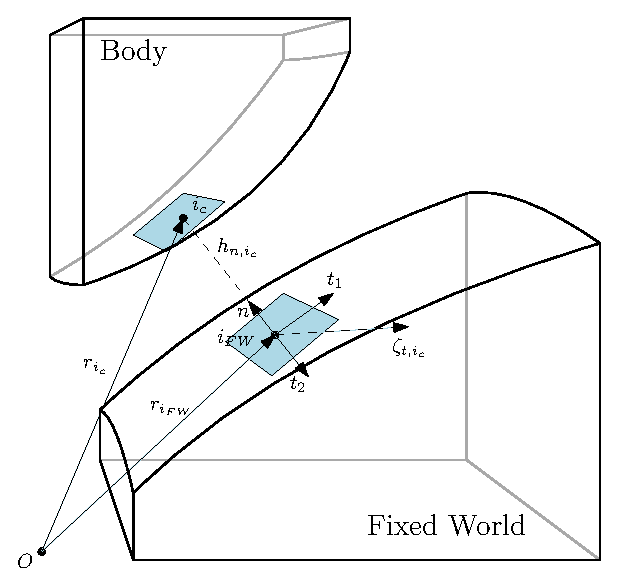
\includegraphics[width=.5\textwidth]{contactplanes.eps}\caption{An illustration of a body impacting the fixed world. A contact point $\iota$ is defined on the body, which can make contact with the fixed world at $i_{FW}$. The points $\iota$ and $i_{FW}$ are connected by a line which is perpendicular to their respective bodies, which is used to define the contact distance $h_{n,\iota}$ and normal contact velocity $\zeta_{n,\iota}$. In the plane tangent to the body's surface, the tangential contact velocity $\zetab_{tw,\iota}$ is defined.} \label{fig:contactplanes}
\end{figure}

Then, the continuous dynamics of a mechanical system with unilateral constraints and spatial friction are of the form
\begin{align}
&\Mb(\qb)\dot{\xib} + \Cb(\qb,\xib) = \Sb(\qb)\ub + \sum_{\iota\in\Ic_{\text{cl}}}\wb_{n,\iota}(\qb)\lambda_{n,\iota} + \Wb_{t,\iota}(\qb)\lambdab_{t,\iota}, \label{eq:appcont1}\\
&\text{(Contact Law)},\nonumber\\
&\text{(Friction Law)},\nonumber
\end{align}
\nomenclature[V]{$\lambda_{n,\iota}$}{The normal reaction force of contact point $\iota$}%
\nomenclature[V]{$\lambdab_{t,\iota}$}{The tangential reaction force of contact point $\iota$}%
\nomenclature[V]{$\Lambda_{n,\iota}$}{The normal impulsive reaction force of contact point $\iota$}%
\nomenclature[V]{$\Lambdab_{t,\iota}$}{The tangential impulsive reaction force of contact point $\iota$}%
\nomenclature[V]{$\Mb$}{The mass matrix}%
\nomenclature[V]{$\Cb$}{The column containing centripedal, Coriolis and gravitational effects}%
\nomenclature[V]{$\Sb$}{The matrix containing generalized directions of the actuator forces}%
with $\qb,\xib\in\Rbb^{n}$ and $\ub\in\Rbb^m$. Here $\Mb(\qb)\in\Rbb^{n\times n}$ is the mass matrix of the system, $\Cb(\qb,\xib)\in\Rbb^{n}$ contains the centripetal, Coriolis and gravitational forces in the system and $\Sb(\qb)\in\Rbb^{n\times m}$ represents the generalized directions of the forces. $\lambda_{n,\iota}\in\Rbb$ and $\lambdab_{t,\iota}\in\Rbb^{2}$ are the normal and tangential reaction forces, respectively, of contact point $\iota$ with $\wb_{n,\iota}\in\Rbb^{n}$ and $\Wb_{t,\iota}\in\Rbb^{n\times 2}$ the corresponding reaction force Jacobians. When a contact point activates a unilateral constraint, impulsive dynamics can cause the state of the system to jump. These dynamics are of the form

\begin{align}
&\Mb(\qb)(\xib^+ - \xib^-) = \sum_{\iota\in\Ic_{\text{cl}}} \wb_{n,\iota}(\qb)\Lambda_{n,\iota} + \Wb_{t,\iota}(\qb)\Lambdab_{t,\iota}, \label{eq:appimp1}\\
&\text{(Impulsive Contact Law)},\nonumber\\
&\text{(Impulsive Friction Law)}.\nonumber
\end{align}
Here $\Lambda_{n,\iota}$ and $\Lambdab_{t,\iota}$ the normal and tangential impulsive reaction forces, respectively, of contact point $\iota$. These dynamics are impulsive, and happen at one instance in time. The $^-$ superscript indicates the ante-event state and the $^+$ superscript indicates the post-event state. In the following sections three different methods of describing the contact and friction laws are presented. First a complementarity problem formulation of mechanical systems with unilateral constraints is given, from which later a proximal point formulation and a hybrid system formulation are derived. For more information on modeling of multibody systems one can refer to \cite{Leine2008} and \cite{Wouw2016}.

\section{Complementarity problem formulation}\label{sec:comp}
\subsection{Signorini's contact law and Poisson's impact law}
To describe the normal contact between rigid bodies Signorini's contact law is used. Since the bodies are impenetrable and reaction forces caused by contact cannot prevent the bodies from seperating, both the contact distance $h_{n,\iota}$ and $\lambda_{n,\iota}$ cannot become negative. Two situations are possible

\begin{enumerate}
\item $h_{n,\iota}=0\ \wedge\ \lambda_{n,\iota} \geq 0$ (closed-contact)
\item $h_{n,\iota}>0\ \wedge\ \lambda_{n,\iota} = 0$ (open-contact)
\end{enumerate}

These situations are illustrated in Figure~\ref{fig:signorinicontact}, where it can be seen that the two situations are orthogonal. This behavior can be summarized in the complementarity condition

\begin{align}
0\leq h_{n,\iota}\ \bot\ \lambda_{n,\iota} \geq 0,\label{eq:signorini}
\end{align}

where the symbol $\bot$ is used to express the orthogonality between $h_{n,\iota}$ and $\lambda_{n,\iota}$. The complementarity condition in \eqref{eq:signorini} is called Signorini's contact law.
\begin{figure}[h]
\centering
\begin{subfigure}{0.3\textwidth}
\centering
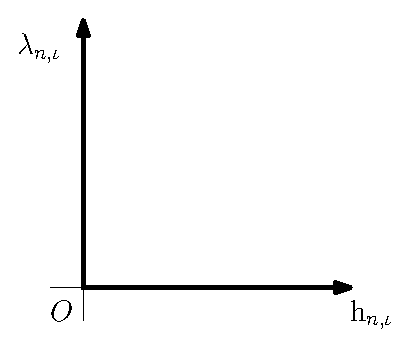
\includegraphics[width=\linewidth]{signorinicontact.eps}
\caption{Signorini's contact law.}\label{fig:signorinicontact}
\end{subfigure}
\qquad
%\begin{subfigure}{0.3\textwidth}
%\centering
%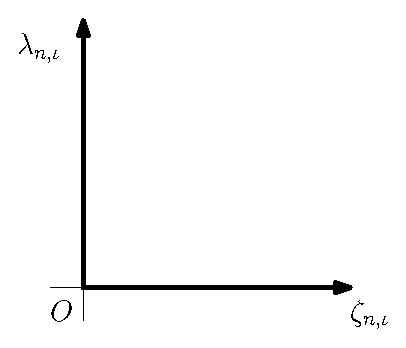
\includegraphics[width=\linewidth]{signoriniforce.eps}
%\caption{Signorini's force law.}\label{fig:signoriniforce}
%\end{subfigure}
%\quad
\begin{subfigure}{0.3\textwidth}
\centering
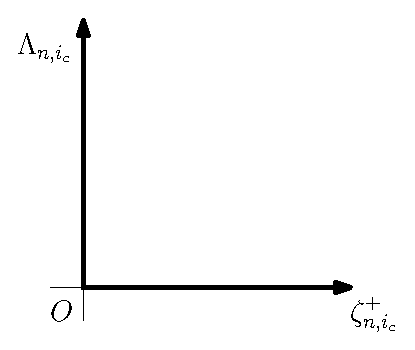
\includegraphics[width=\linewidth]{poissonimpact.eps}
\caption{Poisson's impact law without restitution.}\label{fig:poissonimpact}
\end{subfigure}
\caption{}
\end{figure}
When contact happens at nonzero velocity, impact occurs. Newton's impact law is used to describe this impact. Newton's law of impact is defined as
\begin{align}
\zeta^+_{n,\iota} = -e_{n,\iota}\zeta^-_{n,\iota},\text{ when }h_{n,\iota}=0,\ \dot{h}_{n,\iota}<0.
\end{align}
\nomenclature[P]{$e_{n,\iota}$}{}%
\nomenclature[P]{$e_{t,\iota}$}{}%
In this work the coefficient of restitution $e_{n,\iota}$ is assumed to be $0$, describing a completely inelastic contact. For closed contacts, an impact law can be defined that relates the impulsive contact force $\Lambda_{n,\iota}$ to the post-impact normal velocity $\zeta_{n,\iota}$. Considering multi-contact systems, two situations can occur when a contact is closed:
\begin{enumerate}
\item $\Lambda_{n,\iota} > 0\ \wedge\ \zeta^+_{n,\iota} = 0$ (impact)
\item $\Lambda_{n,\iota} = 0\ \wedge\ \zeta^+_{n,\iota} \geq 0$ (no impact)
\end{enumerate}
The second case can occur when a contact point other than $\iota$ makes impact. The situations described above are illustrated in Figure~\ref{fig:poissonimpact}, where again the orthogonality can be observed. The behavior is written into the complementarity condition
\begin{align}
0\leq \zeta^+_{n,\iota}\ \bot\ \Lambda_{n,\iota} \geq 0,\quad  \qquad \forall \iota\in\Ic_{\text{cl}},\label{eq:poisson}
\end{align}
with $\Ic_{\text{cl}}$ the set of closed contacts. The complementarity condition \eqref{eq:poisson} is called Poisson's impact law. Note that the impact law is defined on velocity level, whereas the contact law is defined on position level.

\subsection{Coulomb's friction law}
Coulomb's friction law is often used to describe dry friction in mechanical systems. When considering 3-dimensional environments, Coulomb's friction law is defined as 
\begin{align}
||\lambdab_{t,\iota}||\ \in\ \left\{ \begin{array}{ll}
||\lambdab_{t,\iota}||\leq\mu_{\iota}\lambda_{n,\iota}, &\text{if }||\zetab_{t,\iota}||=0\\
||\lambdab_{t,\iota}|| = \mu_{\iota}\lambda_{n,\iota}, &\text{if }||\zetab_{t,\iota}||>0
\end{array}\right.,\label{eq:frictionlen}
\end{align}
\nomenclature[P]{$\mu_{\iota}$}{The friction coefficient of contact point $\iota$}%
with $\mu_{\iota}$ the friction coefficient of contact point $\iota$, and since friction is considered isotropic
\begin{align}
\zetab_{t,\iota} = -\kappa_{\iota}\SgnSp(\lambdab_{t,\iota}),\label{eq:frictiondir}
\end{align}
\nomenclature[P]{$\kappa_{\iota}$}{Magnitude of the tangential velocity of contact point $\iota$}
with $\kappa_{\iota}>0$ and
\begin{equation}
\SgnSp(a) = \left\lbrace\begin{array}{ll}
\frac{a}{||a||} & a \neq 0\\
0 & a = 0
\end{array},\right.
\end{equation}
for some vector $a$ as defined in \cite{Studer2006}. \eqref{eq:frictionlen} can be considered as a relation between the magnitude of the tangential velocity $\zetab_{t,\iota}$ and the reaction friction force $\lambdab_{t,\iota}$. \eqref{eq:frictiondir} can be considered as a relation between the direction of $\zetab_{t,\iota}$ and $\lambdab_{t,\iota}$, namely that $\zetab_{t,\iota}$ and $\lambdab_{t,\iota}$ are always in opposite directions. The constant $\kappa_{\iota}$ can then be interpreted as the magnitude of the tangential velocity. Coulomb's friction law is illustrated in Figure~\ref{fig:coulombfriction}. In Figure~\ref{fig:coulombort} the same law is illustrated, but now as orthogonal vectors. As mentioned before, this is convenient for writing the law in a complementarity form.

\begin{figure}[h]
\centering
\begin{subfigure}{0.38\textwidth}
\centering
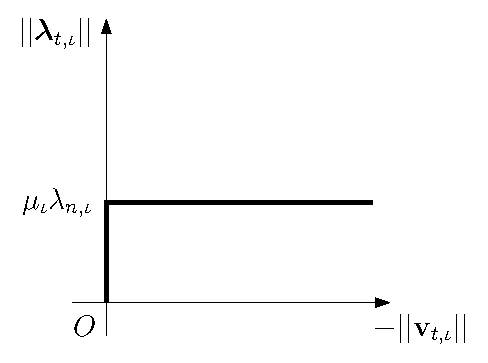
\includegraphics[width=\linewidth]{coulombfriction.eps}\caption{Coulomb's friction law.}\vspace{1.25cm}\label{fig:coulombfriction}
\end{subfigure}
\qquad
\begin{subfigure}{0.3\textwidth}
\centering
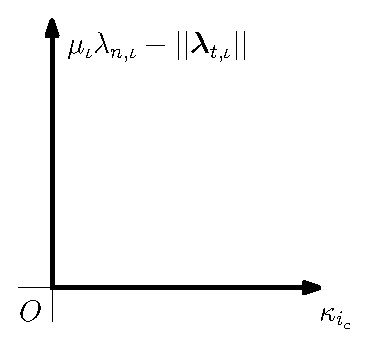
\includegraphics[width=\linewidth]{coulombort.eps}\caption{Coulomb's friction law as orthogonal vectors. $\kappa_{\iota}$ is defined as the magnitude of the tangential velocity $\zetab_{t,\iota}$.}\label{fig:coulombort}
\end{subfigure}
\caption{}
\end{figure}

The complementarity formulation of the Coulomb's law is therefore defined as

\begin{align}
&0\leq \mu_{\iota}\lambda_{n,\iota} - ||\lambdab_{t,\iota}||\ \bot\ \kappa_{\iota} \geq 0,\label{eq:coulomb1}\\
&\zetab_{t,\iota} = -\kappa_{\iota}\SgnSp(\lambdab_{t,\iota}).\label{eq:coulomb2}
\end{align}

\eqref{eq:frictiondir} is rewritten to \eqref{eq:coulomb2} to avoid singularity problems for $||\lambdab_{t,\iota}|| = 0$. For the impulsive behavior of the friction law Newton's impact law is used to define the tangential post-impact velocity as
\begin{align}
\zetab^+_{t,\iota} = -e_{t,\iota}\zetab^-_{t,\iota},
\end{align}
where in this work $e_{t,\iota}=0$ is assumed. Then, similarly to the non-impulsive case, the impulsive Coulomb's friction law can be defined as
\begin{align}
&0 \leq \mu\Lambda_{n,\iota} - ||\Lambdab_{t,\iota}||\ \bot\ \kappa_{\iota} \geq 0. \qquad \forall \iota\in\Ic_{\text{cl}},\label{eq:coulombimp1}\\
&\zetab_{t,\iota}^+ = \kappa_{\iota}\SgnSp(\Lambdab_{t,\iota}),\qquad \forall \iota\in\Ic_{\text{cl}}.\label{eq:coulombimp2}
\end{align}
Note that just as the contact case, the impulsive friction law only holds for closed contacts.
\subsection{System dynamics with contact and friction law}
The flow dynamics are then described by
\begin{align}
&\Mb(\qb)\dot{\xib} + \Cb(\qb,\xib) = \Sb(\qb)\ub + \sum_{\iota\in\Ic_{\text{cl}}}\wb_{n,\iota}(\qb)\lambda_{n,\iota} + \Wb_{t,\iota}(\qb)\lambdab_{t,\iota}, \label{eq:ncpcontact1}\\
&0\leq h_{n,\iota}\ \bot\ \lambda_{n,\iota} \geq 0,\label{eq:ncpcontact2}\\
&0\leq \mu\lambda_{n,\iota} - ||\lambdab_{t,\iota}||\ \bot\ \kappa_{\iota} \geq 0,\label{eq:ncpcontact3}\\
&\zetab_{t,\iota} = -\kappa_{\iota}\SgnSp(\lambdab_{t,\iota}),\label{eq:ncpcontact4}
\end{align}
with 
\begin{align}
&h_{n,\iota} = \wb_{n,\iota}^T(\qb)\qb,\label{eq:h}\\
&\zeta_{n,\iota}(\qb) = \wb^T_{n,\iota}(\qb) \xib,  \label{eq:zetan}\\
&\zetab_{t,\iota}(\qb) = \Wb^T_{t,\iota}(\qb) \xib. \label{eq:zetab}
\end{align}
The discrete dynamics, which take place when a contact point goes through an event, are described by
\begin{align}
&\Mb(\qb)(\xib^+ - \xib^-) = \sum_{\iota\in\Ic_{\text{cl}}} \wb_{n,\iota}(\qb)\Lambda_{n,\iota} + \Wb_{t,\iota}(\qb)\Lambdab_{t,\iota}, \label{eq:ncpimpact1}\\
&0\leq \zeta_{n,\iota}^+\ \bot\ \Lambda_{n,\iota} \geq 0, \qquad \forall \iota\in\Ic_{\text{cl}},\label{eq:ncpimpact2}\\
&0 \leq \mu\Lambda_{n,\iota} - ||\Lambdab_{t,\iota}||\ \bot\ \kappa_{\iota} \geq 0. \qquad \forall \iota\in\Ic_{\text{cl}},\label{eq:ncpimpact3}\\
&\zetab_{t,\iota}^+ = -\kappa^j\SgnSp(\Lambdab_{t,\iota}),\qquad \forall \iota\in\Ic_{\text{cl}},\label{eq:ncpimpact4}
\end{align}
with 
\begin{align}
&\zeta^+_{n,\iota}(\qb) = \wb^T_{n,\iota}(\qb) \xib^+,\\
&\zetab^+_{t,\iota}(\qb) = \Wb^T_{t,\iota}(\qb) \xib^+.\label{eq:ncpimpactend}
\end{align}

\section{Hybrid system formulation}
In this section the dynamics of the complementarity system defined in Section~\ref{sec:comp} is written to a hybrid formulation, resulting in a hybrid framework for mechanical systems with unilateral constraints and spatial friction. In \cite[p. 222]{Acary2008} event driven numerical methods are presented for mechanical systems with spatial friction. However, these methods do not apply to the hybrid system framework. To the best of our knowledge, this work is first in presenting a model suitable for event driven simulation methods for the hybrid system framework with spatial friction.

\nomenclature[V]{$\sigma_j$}{The system-mode descriptor of event $j$}%
\subsection{Hybrid systems with impulsive effects}\label{sec:2hyb}
According to \cite{Haddad2006}, an impulsive dynamical system can be described by a hybrid system with impulsive effects. This makes it a valid framework for mechanical systems with unilateral constraints and spatial friction. The notation given in \cite{Haddad2006} is convenient from a tracking point-of-view, considering that only the dynamics encountered during the trajectory need to be described. A hybrid system with impulsive effects consists of three elements:
\begin{enumerate}
\item Continuous dynamics, a continuous-time differential equation which defines the behavior of the system in between events
\item Discrete dynamics, which defines the way the state of the system is reset during events
\item Reset sets, which is a criterion to decide when the state of the system is to be reset
\end{enumerate}

Therefore, a hybrid system with impulsive effects is given by
\begin{equation}
\begin{array}{ll}
\dot{\xb}(t,j) =\fb(\xb(t,j),\ub(t,j),t,j),& \xb(t,j),\ub(t,j)\in \mathcal{C}^j\\
\xb(t,j+1) = \gb(\xb(t,j),\ub(t,j),t,j),& \xb(t,j),\ub(t,j)\in \mathcal{D}^{j+1}
\end{array}\label{eq:hybimp}
\end{equation}
\nomenclature[V]{$\fb$}{A nonlinear continuous function}%
\nomenclature[V]{$\gb$}{A jump map}%
\nomenclature[V]{$\mathcal{D}$}{A discrete event set}%
\nomenclature[V]{$\gamma$}{A flow guard function}%
\nomenclature[V]{$\Gamma$}{An impulsive guard function}%
\nomenclature[V]{$\alphab$}{The nominal reference trajectory}%
\nomenclature[V]{$\mub$}{The nominal reference input}%
with $\xb(t,j)\in\Rbb^{n(j)}$, $\ub(t,j)\in\Rbb^{m(j)}$, $\fb\ :\ \Rbb^{n(j)}\ \times\ \Rbb^{m(j)}\ \times\ \Rbb\rightarrow \Rbb^{n(j)}$. Note that the state dimension $n(j)$ and the input dimension $m(j)$ can vary in different modes $j$. For the difference equation we have $\gb\ :\ \Rbb^{n(j-1)}\ \times\ \Rbb^{m(j-1)}\ \times\ \Rbb\rightarrow \Rbb^{n(j)}$. $\mathcal{C}^j$ is the flow set of the system, and $\mathcal{D}^j(t) \subseteq \partial \mathcal{C}^j := \{\xb(t,j)\in\Rbb^{n(j)},\ \ub(t,j)\in\Rbb^{m(i)}\ |\ \gamma_{=}^j(\xb^{\wedge},\ub^{\wedge},t) = 0, \ \gamma_{\geq}^j(\xb^{\wedge},\ub^{\wedge},t) \geq 0\}$, where $\gamma_{=}^j$ and $\gamma_{\geq}^j$ are some sets of guard functions that are activated at event $j$, $\xb^{\wedge}$,$\ub^{\wedge}$ are some virtual state and input that are not necessarily physically realistic, and $\partial \mathcal{C}^j$ indicates the border of $\mathcal{C}^j$.

The dynamics given in \eqref{eq:hybimp} will be used to describe a tracking problem for mechanical systems with unilateral constraints and spatial friction. A nominal state-input trajectory is considered consisting of absolutely continuous segments $(\alphab(t,j),\mub(t,j))$, with $t\in\left[\tau^j,\tau^{j+1}\right]$ and $j\in\{0,1,...,N\}$ the event counter. The nominal state and input, $\alphab(t,j)$ and $\mub(t,j)$ respectively, define the nominal trajectory with $N$ events. The nominal event time of event $j$ is denoted by $\tau^j$ and regular time is denoted by $t$. Every segment of the nominal trajectory $(\alphab(t,j),\mub(t,j))$ and every event $j\in\{1,2,...,N\}$ satisfy the dynamics in \eqref{eq:hybimp}, where an event happens when $(\alphab(t,j),\mub(t,j))$ enters $\mathcal{D}^{j+1}$. Such a nominal trajectory existing of absolutely continuous segments experiencing events according to \eqref{eq:hybimp} is illustrated in Figure~\ref{fig:2exampletraj}.

In \ref{fig:2example} an example trajectory of a block pushing towards a surface is illustrated. The block has two contact points on its edges $\iota_1$ and $\iota_2$. It starts with both contact points in open contact as can be seen in Figure~\ref{fig:2example1}. The flow is described by $\dot{\alphab}(t,0) = \fb^0(\alphab(t,0),\mub(t,0),t)$ for $t\in[t_0,\tau^1]$. Then $i_2$ makes impact with the surface at $\tau^1$, causing a jump in the state and a change in continuous dynamics $\dot{\alphab}(t,1) = \fb^1(\alphab(t,1),\mub(t,1),t)$ for $t\in[\tau^1,\tau^2]$. This is illustrated in Figure~\ref{fig:2example2}, where $i_2$ is in closed contact and slipping over the contact surface. At $\tau^2$, $i^1$ makes impact as well causing another jump and another change in continuous dynamics. The block now has both contact points slipping over the contact surface. After this both contact points release contact one by one. Since there are no impulsive forces present in this transition, the state does not jump when a contact point releases. However, a jump in the time-derivate of the state is possible, which makes these transitions continuous but nonsmooth.

\begin{figure}[h]
\centering
\begin{subfigure}[b]{0.17\textwidth}
\centering
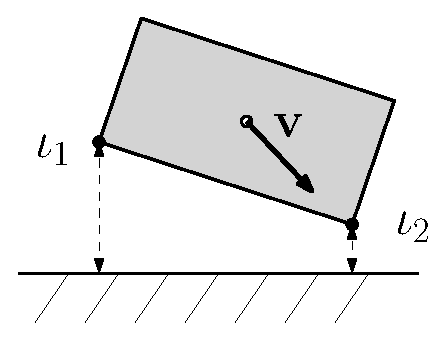
\includegraphics[width=\textwidth]{example1.eps}
\caption{$\iota_1,\iota_2\in\Ic_{\text{op}}$}
\label{fig:2example1}
\end{subfigure}
\quad
\begin{subfigure}[b]{0.17\textwidth}  
\centering 
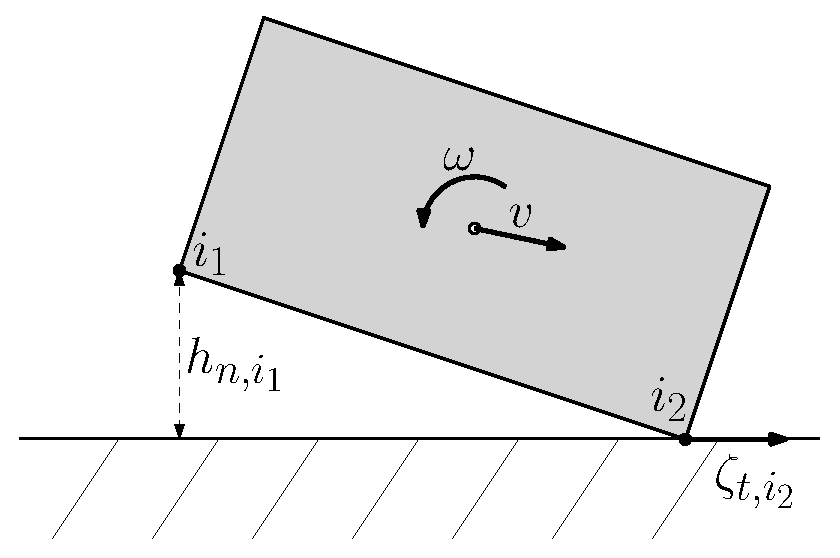
\includegraphics[width=\textwidth]{example2.eps}
\caption{$\iota_2\in\Ic_{\text{sl}}$}
\label{fig:2example2}
\end{subfigure}
\quad
\begin{subfigure}[b]{0.17\textwidth}   
\centering 
\includegraphics[width=\textwidth]{example3.eps}
\caption{$\iota_1,\iota_2\in\Ic_{\text{sl}}$}
\label{fig:2example3}
\end{subfigure}
\quad
\begin{subfigure}[b]{0.17\textwidth}  
\centering 
\includegraphics[width=\textwidth]{example4.eps}
\caption{$\iota_1\in\Ic_{\text{sl}}$}
\label{fig:2example4}
\end{subfigure}
\quad
\begin{subfigure}[b]{0.17\textwidth}   
\centering 
\includegraphics[width=\textwidth]{example5.eps}
\caption{$\iota_1,\iota_2\in\Ic_{\text{op}}$}
\label{fig:2example5}
\end{subfigure}
\vskip\baselineskip
\begin{subfigure}[b]{\textwidth}   
\centering 
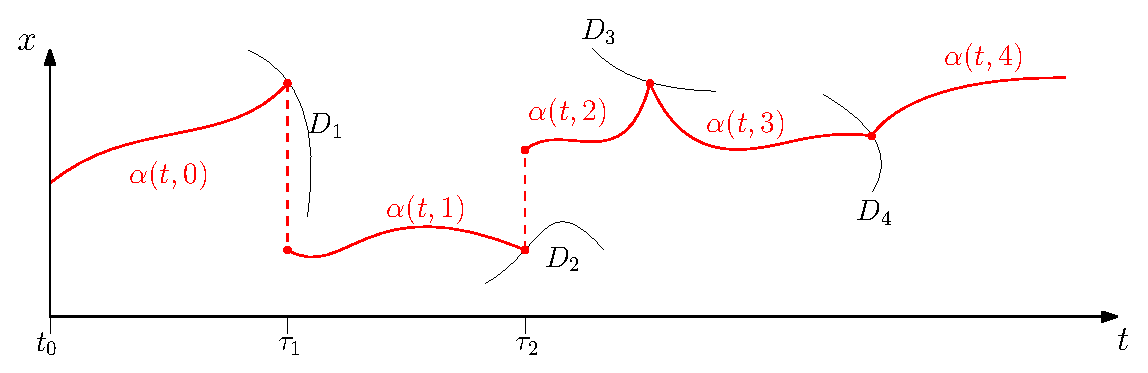
\includegraphics[width=.85\textwidth]{exampletraj1.eps}
\label{fig:2exampletraj}
\end{subfigure}
\caption{An example trajectory, which satisfies the dynamics \eqref{eq:hybimp}, of a block pushing towards and withdrawing from a surface with velocity $v$.  Note that the sets $D$ besides being dependent on $\xb$, are also dependent on $\ub$. Also, although not depicted in this image, the state space of the system varies with every event.}
\label{fig:2example}
\end{figure}

The following sections will be used to write the complementarity system defined in Section~\ref{sec:comp} into a hybrid system with impulsive effects as in \eqref{eq:hybimp}. In \ref{sec:2contdyn} the continuous dynamics $\fb^j$ will be derived for mechanical systems with unilateral constraints and spatial friction. Then, in Section~\ref{sec:2event} the reset set $\mathcal{D}^j$ will be defined. Finally, in Section~\ref{sec:2discdyn} the discrete dynamics $\gb^j$ will be derived. This will fully define the hybrid system with impulsive effects formulation of mechanical systems with unilateral constraints and spatial friction.

\subsection{Continuous dynamics}\label{sec:2contdyn}
When describing mechanical systems, we take 

\begin{align}
\xb = \begin{bmatrix}
\qb\\ \dot{\qb}
\end{bmatrix},\quad
\dot{\xb} = \begin{bmatrix}
\dot{\qb}\\ \ddot{\qb}
\end{bmatrix},
\end{align}

where $\qb$ and $\dot{\qb}$ are the joint positions, velocities and accelerations respectively. As described in Section~\ref{sec:comp}, for mechanical systems a set of contact points $\iota\in\{\iota_1,\iota_2,...,\iota_c\}$ is defined. Here $c$ is the number of considered contact points. A set $\Ic_{\text{cl}}$ is defined as the set of closed contact points, such that a contact $\iota\in\Ic_{\text{cl}}$ has closed a unilateral constraint. The set of contact points in open contact is defined as $\Ic_{\text{op}} := \{\iota\ |\ \iota\notin\Ic_{\text{cl}}\}$. The set $\Ic_{\text{cl}}$ is subdivided in two subsets $\Ic_{\text{sl}}$ and $\Ic_{\text{st}}$, where $\Ic_{\text{sl}}$ is the set of closed contact points in slip and $\Ic_{\text{st}}$ the set of closed contact points in stick. Here $\Ic_{\text{cl}} =\Ic_{\text{sl}}\cup\Ic_{\text{st}}$ and $\Ic_{\text{sl}}\cup\Ic_{\text{st}}=\emptyset$. 

The equations of motion, given in \eqref{eq:appcont1}, can be rewritten to
\begin{align}
\ddot{\qb} = \Mb^{-1}(\qb)\left[ \Sb(\qb)\ub - \Cb(\qb,\dot{\qb}) + \Wb_{n}(\qb)\lambdab_{n} + \Wb_{t}(\qb)\lambdab_{t}\right],\label{eq:qddot}
\end{align}
with
\begin{align}
\Wb_n &= \begin{bmatrix}
\wb_{n,i_1},\wb_{n,i_2},...,\wb_{n,\iota}
\end{bmatrix}\in\Rbb^{n\times c},\\
\Wb_t &= \begin{bmatrix}
\Wb_{t,i_1},\Wb_{t,i_2},...,\Wb_{t,\iota} 
\end{bmatrix}\in\Rbb^{n\times 2c},\\
\lambdab_n &= \begin{bmatrix}
\lambda_{n,\iota_1};\lambda_{n,\iota_2};...;\lambda_{n,\iota_c} 
\end{bmatrix}\in\Rbb^{c},\\
\lambdab_t &= \begin{bmatrix}
\lambdab_{t,\iota_1};\lambdab_{t,\iota_2};...;\lambdab_{t,\iota_c} 
\end{bmatrix}\in\Rbb^{2c},
\end{align}
Note that since $\fb^j$ is only defined on $\xb(t,j),\ub(t,j)\notin \mathcal{D}^j$, it is not necessary to use $\xib$ to define the equations of motion as done in \eqref{eq:appcont1}. Now $\fb^j$ can be written as
\begin{align}
\dot{\xb}(t,j) =\begin{bmatrix}
\dot{\qb}\\ \Mb^{-1}(\qb)\left[ \Sb(\qb)\ub - \Cb(\qb,\dot{\qb}) + \Wb_{n}(\qb)\lambdab_{n} + \Wb_{t}(\qb)\lambdab_{t}\right]
\end{bmatrix}.\label{eq:fcont}
\end{align}
The closed contact points in $\Ic_{\text{cl}}$ experience reaction forces $\lambda_{n,\iota}$ and $\lambdab_{t,\iota}$, as can be seen in \eqref{eq:qddot}. Therefore for all closed contact points $\iota\in\Ic_{\text{cl}}$ constraints are given which define these reaction forces. These constraints are given by
\begin{align}
&\wb^T_{n,\iota}(\qb)\ddot{\qb} + \dot{\wb}^T_{n,\iota}(\qb)\dot{\qb} = 0, &\forall \iota\in\Ic_{\text{cl}},\label{eq:fcontconst1}\\
&\lambdab_{t,\iota} + \mu_{\iota}\lambda_{n,\iota}\SgnSp(\Wb_{t,\iota}^T\dot{\qb}) = 0, &\forall \iota\in\Ic_{\text{sl}},\label{eq:fcontconst2}\\
&\Wb^T_{t,\iota}(\qb)\ddot{\qb} + \dot{\Wb}^T_{t,\iota}(\qb)\dot{\qb} = 0, &\forall \iota\in\Ic_{\text{st}},\label{eq:fcontconst3}
\end{align}
where $\Ic_{\text{sl}}$ and $\Ic_{\text{st}}$ are the sets of closed contacts in slip and closed contacts in stick respectively. Now, with \eqref{eq:fcont} and \eqref{eq:fcontconst1}-\eqref{eq:fcontconst3}, the continuous dynamics of the hybrid system with impulsive dynamics are correctly defined. A more thorough derivation of these dynamics can be found in Appendix~\ref{app:hybrid}.

\textbf{System mode descriptor}\\
A system will have different flow dynamics as the system mode changes, as can be seen in \eqref{eq:fcontconst1}-\eqref{eq:fcontconst3}. Also the guard functions that can be activated will change with the mode, as will be shown in Section~\ref{sec:2event}. Therefore it is necessary to keep track of the mode the system is in. The system mode descriptor $\sigma^j$ is introduced to conveniently describe the current system mode. Each contact point can either be in open-contact, closed-contact slip or closed-contact stick. The system mode descriptor is therefore defined as the ordered set
\begin{align}
\sigma = (\sigma_1,\sigma_2,...,\sigma_\iota),
\end{align}
\nomenclature[V]{$\sigma$}{The system mode descriptor}
where $\sigma_\iota$ is the mode of contact point $\iota$. $\sigma_\iota$ can either have the value `op' for a contact point in open-contact, `sl' for a contact point in closed-contact slip, or `st' for a contact point in closed-contact stick. For example, the system mode descriptor of the mode in Figure~\ref{fig:2example2} is $\sigma = \{\text{op},\text{sl}\}$.

\subsection{Discrete event sets}\label{sec:2event}
When the continuous dynamics enter an event set $\mathcal{D}$, an event will take place. Such an event can cause a contact point to enter a different set. This will lead to different post-event continuous dynamics, and it can cause the state to reinitialize according to the discrete dynamics presented in Section~\ref{sec:2discdyn}. For each set of contact points these sets are defined differently. In this section the sets $\mathcal{D}$ are defined for each set of contact points. The derivation of the discrete event sets can be found in Appendix~\ref{app:hybrid}.

\textbf{Discrete events sets in open contact}\\
For all contact points $\iota\in\Ic_{\text{op}}$ the discrete event sets are defined as
\begin{align}
\mathcal{D}^{\text{op}\rightarrow\text{cl}}_{\iota} &= \{ \qb\ |\ \gamma^{\text{op}\rightarrow\text{cl}}_{\iota} = 0,\ \dot{\gamma}^{\text{op}\rightarrow\text{cl}}_{\iota} < 0 \},\label{eq:2Dopcl}
\end{align}
\nomenclature[V]{$\mathcal{D}^j$}{The discrete event set of event $j$}%
with
\begin{align}
\gamma^{\text{op}\rightarrow\text{cl}}_{\iota} &= h_{n,\iota}(\qb).
\end{align}


\textbf{Discrete events sets in closed contact slip}\\
For all contact points $\iota\in\Ic_{\text{sl}}$ the discrete event sets are defined as
\begin{align}
\mathcal{D}^{\text{sl}\rightarrow\text{st}}_{\iota} &= \{ \qb\ |\ \gamma^{\text{sl}\rightarrow\text{st}}_{\iota} = 0,\ \dot{\gamma}^{\text{sl}\rightarrow\text{st}}_{\iota} < 0\},\label{eq:2Dslst}\\
\mathcal{D}^{\text{cl}\rightarrow\text{op}}_{\iota} &= \{ \qb,\ub\ |\ \gamma^{\text{cl}\rightarrow\text{op}}_{\iota} = 0,\ \dot{\gamma}^{\text{cl}\rightarrow\text{op}}_{\iota} < 0\},\label{eq:2Dslop}
\end{align}
with 
\begin{align}
\gamma^{\text{sl}\rightarrow\text{st}}_{\iota} &= \sqrt{\zetab_{t,\iota}\zetab_{t,\iota}^T},\\
\gamma^{\text{cl}\rightarrow\text{op}}_{\iota} &= \lambda_{n,\iota}.
\end{align}

\textbf{Discrete events sets in closed contact stick}\\
For all contact points $\iota\in\Ic_{\text{st}}$ the discrete event sets are defined as
\begin{align}
\mathcal{D}^{\text{st}\rightarrow\text{sl}}_{\iota} &= \{ \qb,\ub\ |\ \gamma^{\text{st}\rightarrow\text{sl}}_{\iota} = 0,\ \dot{\gamma}^{\text{sl}\rightarrow\text{st}}_{\iota} < 0\},\label{eq:2Dstsl}\\
\mathcal{D}^{\text{cl}\rightarrow\text{op}}_{\iota} &= \{ \qb,\ub\ |\ \gamma^{\text{cl}\rightarrow\text{op}}_{\iota} = 0,\ \dot{\gamma}^{\text{cl}\rightarrow\text{op}}_{\iota} < 0\},\label{eq:2Dstop}
\end{align}
with 
\begin{align}
\gamma^{\text{st}\rightarrow\text{sl}}_{\iota} &= \mu^2\lambda_{n,\iota}^2-\lambdab_{t,\iota}\lambdab_{t,\iota}^T,\\
\gamma^{\text{cl}\rightarrow\text{op}}_{\iota} &= \lambda_{n,\iota}.
\end{align}
These event sets lead to a non-impulsive event, which is described in Section~\ref{sec:2discdyn}.

\subsection{Discrete dynamics}\label{sec:2discdyn}
A contact point entering a discrete event set $\mathcal{D}$ indicates that the system in its current mode is infeasible. The system should therefore go through a discrete event, in which the state can be reinitialized and the mode can be changed to a feasible system. One contact point entering a discrete event set can lead to other contact points experiencing infeasible reaction forces, making it difficult to determine in what mode each contact point should be. The reinitialization of the state and selection of a post-event mode is described by the discrete dynamics in this section. First a \textit{nonlinear complementarity problem} (NCP) is solved to reinitialize the state. The NCP generates a unique feasible solution \cite{Delassus1917}, which for simple systems can be found by iterating over all solutions until the feasible solution is found. Then a mode selection algorithm is presented to find a feasible post-event mode, which defines the continuous dynamics to be integrated after the event. 
\nomenclature[A]{NCP}{Nonlinear Complementarity Problem}%

\textbf{State reinitialization}\\
From the impulsive dynamics \eqref{eq:ncpimpact1}-\eqref{eq:ncpimpact4}, the discrete dynamics for an impulsive event which determine the post-event state $\qb^+$ can be derived as
\begin{align}
\dot{\qb}^+ &= \Mb^{-1}\left[\Wb_{n}\Lambdab_{n} + \Wb_{t}\Lambdab_{t}\right] + \dot{\qb}^-, \label{eq:2ncp1}\\
\wb^T_{n,\iota}\dot{\qb}^+ &= 0, &\forall \iota\in\Ic_{\text{cl}},\label{eq:2ncp2}\\
\Lambdab_{t,\iota} + \mu\Lambda_{n,\iota}\SgnSp(\zetab^-_{t,\iota})&= 0, &\forall \iota\in\Ic_{\text{sl}},\label{eq:2ncp3}\\
\Wb^T_{t,\iota}\dot{\qb}^+ &= 0, &\forall \iota\in\Ic_{\text{st}}.\label{eq:2ncp4}
\end{align}
Here the unknown variables are $\dot{\qb}^+\in\Rbb^{n}$, $\Lambdab_{n}\in\Rbb^{c_{\text{cl}}}$ and $\Lambdab_{t}\in\Rbb^{2c_{\text{cl}}}$, which means that there are $n+3c_{\text{cl}}$ unknown variables. From \eqref{eq:2ncp1} we get $n$ equations, from \eqref{eq:2ncp2} we get $c_{\text{cl}}$ equations and since $\Ic_{\text{sl}}\cup\Ic_{\text{st}}=\Ic_{\text{cl}}$, $\lambdab_{t,\iota}\in\Rbb^2$, and $\Wb^T_{t,\iota}\ddot{\qb}^+ + \dot{\Wb}^T_{t,\iota}\dot{\qb}^+ \in\Rbb^2$ we get $2c_{\text{cl}}$ equations from \eqref{eq:2ncp3}-\eqref{eq:2ncp4}. Since we have $n+3c_{\text{cl}}$ unknown variables and $n+3c_{\text{cl}}$ equations, the system is solvable.

The problem that remains is that it is not straightforward to know which dynamics to solve, because the dynamics change as the system-mode changes. The set of equations that should be solved is the set of equations that corresponds to the system-mode which generates a feasible post-event state. When a contact point enters a discrete event set, and thus generates an infeasible state, it can be concluded that the system will go through an event because in it's current mode the system is infeasible. However, it is not guaranteed that the contact point which entered the event set will change their mode. Actually any contact point, or even several contact points, can change their mode. Therefore the dynamics should be solved for several modes, until a feasible post-event state is found. A feasible post-event state is a post-event state solved for a certain system-mode $\sigma$, such that the all corresponding guard functions are in its unactivated state, i.e., all $\Gamma_{\iota}>0$. As mentioned earlier, there will exist a unique system-mode where the system has a feasible post-impact state. Similar to the non-impulsive guard functions defined in Section~\ref{sec:2event}, the impulsive guard functions are given by
\begin{align}
\Gamma^{\text{cl}\rightarrow\text{op}}_{\iota} &= \Lambda_{n,\iota},\\
\Gamma^{\text{sl}\rightarrow\text{st}}_{\iota} &= \zetab^+_{t,\iota}(\zetab^+_{t,\iota})^T,\\
\Gamma^{\text{st}\rightarrow\text{sl}}_{\iota} &= \mu^2\Lambda_{n,\iota}^2 - \Lambdab_{t,\iota}\Lambdab_{t,\iota}^T.
\end{align}
Note that all guard functions are defined at velocity level during the state reinitialization. The NCP is defined at velocity level, meaning that only guard functions on velocity level need to be considered. For example, it is impossible for the state reinitialization to generate an infeasible position because the position of the system is not updated during the state reinitialization. When $\Lambda_{n,\iota} = 0$ and $\Lambdab_{t,\iota} = 0$ during an event, one speaks of a non-impulsive event. In this case the state is not reinitialized during the event. However, the system will enter a different mode however. For both impulsive and non-impulsive events the post-event mode is determined during the mode selection, which is described below.

\textbf{Mode selection}\\
The mode $\sigma$ of a system is determined by the guard functions defined in Section~\ref{sec:2event}. All guard functions $\gamma_\iota$ should be greater than zero for the system to be in a feasible mode. Because some of these guard functions are defined on acceleration level and the post-event acceleration is not constrained by the NCP, we should first find a post-event mode $\sigma^+$ where the accelerations $\ddot{\qb}$ and reaction forces $\lambdab_{n},\lambdab_{t}$ are feasible before we know which continuous dynamics describe a feasible system. From the continuous dynamics \eqref{eq:ncpcontact1}-\eqref{eq:ncpcontact4}, post-event accelerations and reaction forces are defined by
\begin{align}
\ddot{\qb}^+ &= \Mb^{-1}\left[\Sb\ub^+ - \Cb + \Wb_{n}\lambdab^+_{n} + \Wb_{t}\lambdab^+_{t}\right], &  \label{eq:2nonimp1}\\
\wb^T_{n,\iota}\ddot{\qb}^+ + \dot{\wb}^T_{n,\iota}\dot{\qb}^+ &= 0, & \forall \iota\in\Ic_{\text{cl}},\label{eq:2nonimp2}\\
\lambdab^+_{t,\iota} + \mu\lambda^+_{n,\iota}\SgnSp(\Wb_{t,\iota}^T\dot{\qb}^+) &= 0, & \forall \iota\in\Ic_{\text{sl}},\label{eq:2nonimp3}\\
\Wb^T_{t,\iota}\ddot{\qb}^+ + \dot{\Wb}^T_{t,\iota}\dot{\qb}^+ &= 0, & \forall \iota\in\Ic_{\text{st}},\label{eq:2nonimp4}
\end{align}
where $\Mb$, $\Sb$, $\Cb$, $\wb_{n,\iota}$ and $\Wb_{t,\iota}$ are evaluated at the post-event state $\qb^+$ and state time-derivative $\dot{\qb}^+$. Because we are interested in whether the accelerations and reaction forces are feasible, the guard functions defined on acceleration level are evaluated. The guard functions that determine the feasibility of a post-event mode are given by
\begin{align}
\gamma^{\text{cl}\rightarrow\text{op}}_{\iota}(\ddot{\qb}) &= \lambda_{n,\iota}, & \forall \iota\in\Ic_{\text{cl}},\\
\gamma^{\text{st}\rightarrow\text{sl}}_{\iota}(\ddot{\qb}) &= \mu_{\iota}^2\lambda_{n,\iota}^2 - \lambdab_{t,\iota}\lambdab_{t,\iota}^T, & \forall \iota\in\Ic_{\text{st}},
\end{align}
with $\Ic_{\text{sl}}\cup\Ic_{\text{st}}=\Ic_{\text{cl}}$. Note that the guard functions $\gamma_{\iota}^{\text{op}\rightarrow\text{cl}}$ and $\gamma_{\iota}^{\text{sl}\rightarrow\text{st}}$ are not evaluated. This is unnecessary, because contact points in open contact can only activate guard functions defined at position level. Since the non-impulsive dynamics only update the acceleration, it is impossible for a contact point in open contact to change mode during an impulsive event. This also holds for the guard function from slip to stick, which is defined on velocity level.

The process of solving a hybrid system with impulsive effects is illustrated in Figure~\ref{fig:2hybridalg}. The system first flows according to some continuous dynamics. When an event set $\mathcal{D}$ is entered, the system gives a ante-event state $\xb^-$. Then during the state reinitialization an NCP is solved using the ante-event state, which determines the post-event state $\xb^+$. Finally, the mode selection is solved, which finds a feasible post-event mode $\sigma^+$ for that post-event state $\xb^+$. The continuous dynamics for the next flow segment is defined by $\sigma^+$ with $\xb^+$ the initial condition.

\begin{figure}[h]
\centering
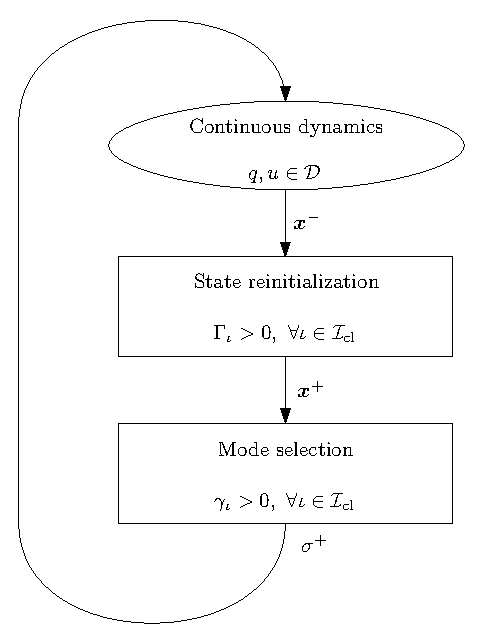
\includegraphics[width=.35\textwidth]{hybridalg.eps}\caption{The algorithm used to solve a hybrid system with impulsive effects depicted in a flowchart.} \label{fig:2hybridalg}
\end{figure}

\section{Summary}
The modeling of mechanical systems with unilateral constraints and spatial friction is presented in this chapter. First a complementarity problem formulation of such systems is presented, using Signorini's contact law, Poisson's impact law and Coulomb's friction law. This system fully defines the dynamics of mechanical systems with unilateral constraints and spatial friction. From the complementarity problem formulation a hybrid system with impulsive effects is derived. This system is defined with a control point-of-view in mind, and its compatibility with the control strategy that will be presented in the following chapters. The hybrid system is defined in three parts. First the continuous dynamics are presented. Then the discrete event sets are given, which are state-input sets that trigger a discrete event when the state and input enters such a set. Finally the dynamics of such an event are presented, which consist of a state reinitialization and a mode selection.
\end{document}